\documentclass{article}

\usepackage[margin=1in]{geometry}
\usepackage{graphicx} % Allow image/pdf includes
\usepackage{extramarks} % Extra header marks (continued on next page)
\usepackage{amsmath} % Math enhancements
\usepackage{amsthm} % Theorem typesetting
\usepackage{amssymb} % Extended symbol collection
\usepackage{tikz} % Graphical element creation
\usetikzlibrary{automata,positioning}
\usepackage[plain]{algorithm} % Float wrapper for algorithms
\usepackage{algpseudocode} % Algorithm layout
\usepackage{enumitem} % Enumerate (lists)
\usepackage{ragged2e} % Alternative alignment
\usepackage{gensymb} % Generic symbols (degree, etc)
\usepackage{empheq} % Allow \boxed around \begin{empheq}
\usepackage{color,soul} % Highlighting
\usepackage{booktabs} % Enhanced table creation
\usepackage{multirow} % Table multi row
\usepackage{mathtools} % Math enhancements
\usepackage{bm} % Bold math
\usepackage[mathscr]{euscript} % Script variables
\usepackage{cancel} % Cancel through text
\usepackage{color,soul} % Highlighting
\usepackage{mathtools}
\usepackage{multirow}
\usepackage{mathrsfs}
\usepackage{physics}
\usepackage{gensymb}
\usepackage{siunitx}
\usepackage[cache=false]{minted}
\renewcommand{\MintedPygmentize}{/Users/loganharbour/miniconda/bin/pygmentize}

\setlength\parindent{0pt} % No indents
\setlength{\parskip}{1em} % Paragraph skip

\newcommand{\vx}{\mathbf{x}} % x vector
\newcommand{\vy}{\mathbf{y}} % x vector

\newcommand{\pageTitle}{MEEN 644 - Homework 1}
\newcommand{\pageAuthor}{Logan Harbour}

\begin{document}

\title{\LARGE \textbf{\pageTitle} \vspace{-0.3cm}}
\author{\large \pageAuthor}
\date{\vspace{-0.6cm} \large \today \vspace{-0.4cm}}

\maketitle

\section*{Problem statement}

Consider an oscillation of a simple pendulum of length $l$ and mass $m$. The equation of motion is described by
\[
	m \frac{d^2 \theta}{d t^2} + \frac{mg \sin \theta}{\ell} = 0\,,
\]
where $m = 1$ kg and $\ell = 1$ m.

The pendulum is initially displaced to $20^\circ$, and let go from the rest position to oscillate. Assume that there is no friction and the oscillation is not damped.
\begin{enumerate}[label=(\alph*)]
	\item (50 points) Starting with $\Delta t = 0.5$ sec as the time step of integration, calculate displacement (radians) and angular velocity in rad/s using the Runge-Kutta Second Order method. Stop your calculation at the end of one cycle.
	\item (20 points) Continue calculations made in (a) by systematically decreasing the step size $\Delta t$ by half. Declare grid independence when the relative change in displacement and angular velocity with successive time steps vary less than $10^{-4}$. Plot your results.
	\item (30 points) Use the $\Delta t$ corresponding to the grid independent solution (b). Calculate displacement and angular velocity for one cycle using Euler explicit and Euler implicit methods.
\end{enumerate}

\section*{Preliminaries}

\subsection*{Problem reduction}

We define a new variable $\omega = \frac{d \theta}{dt}$ to obtain the reduced system
\begin{equation}
	\begin{cases}
		\frac{d\theta}{dt} = \omega = f_1(t, \vy)\,,\\
		\frac{d\omega}{dt} = - \frac{g}{\ell} \sin \theta = f_2(t, \vy)\,,\\
		\theta(0) = \theta_0 = 20^\circ = \frac{\pi}{9}\,,\\
		\omega(0) = \omega_0 = 0\,,
	\end{cases}
\end{equation}
where $\vy = [\theta, \omega]^T$, $\vy_0 = [\theta_0, \omega_0]^T$, $\mathbf{f}(t, \vy) = [f_1(t, \vy), f_2(t, \vy)]^T$, and $g = 9.81$.

\subsection*{Discretization}

We first define a step size $\Delta t$ with $t_i = i \Delta t$ and $\vy_i = \vy(t_i)$. A full period (computed using the small-angle approximation) is $T = 2 \pi \sqrt{\frac{\ell}{g}} \approx 2.006$ s, therefore a final time was chosen as 2.0 s to allow for only four timesteps with the intial timestep size of $\Delta t = 0.5$ s.

The discretized equations are as follows.

\begin{itemize}
	\item Runge-Kutta second order:
	\begin{subequations}
		\begin{equation}
			\mathbf{k}_{1,n} = \mathbf{f}(t_n, \vy_n)\,,
		\end{equation}
		\begin{equation}
			\mathbf{k}_{2,n} = \mathbf{f}(t_{n+1}, \vy_n + \Delta t \mathbf{k}_{1,n})\,,
		\end{equation}
		\begin{equation}
			\vy_{n+1} = \vy_n + \frac{\Delta t}{2} (\mathbf{k}_{1,n} + \mathbf{k}_{2,n})
		\end{equation}
	\end{subequations}

	\item Explicit Euler:
	\begin{equation}
		\vy_{n+1} = \vy_n + \Delta t \mathbf{f}(t_n, \vy_n)\,,
	\end{equation}

	\item Implicit Euler:
	\begin{equation}
		\vy_{n+1} = \vy_n + \Delta t \mathbf{f}(t_{n+1}, \vy_{n+1}) \,,
	\end{equation}
	which was solved for $\vy_{n+1}$ using a non-linear solver; in specific, the Newton solver \texttt{fsolve} that is packaged in \texttt{SciPy} with an initial guess of $\vy_n$.
\end{itemize}

\subsection*{Grid independence}

First, we define a relative change between successive timestep sizes as
\[
	\mathrm{relative~change} = \frac{|y_{i,n}^{l+1} - y_{i,n}^l|}{|y_{i,n}^l|}\,,
\]
which compares the solution of variable $i$ at time $t_n$ between evaluations where the timestep was at $l$ and $l+1$. For example, for $l$ corresponding to a timestep of $\Delta t = 0.5$ s, $l + 1$ would correspond to a timestep of $\Delta t = 0.25$ s. For a timestep with index $l + 1$, this value is computed for every variable and every solution time that is common with the solution times of timestep index $l$. This is therefore an appropriate representation of the change of the solution between successive timesteps as requested, as it takes into account the convergence of the solution over the entire time $t = [0, 2]$ s. We then stop computation when the maximum of all of the relative changes is $< 10^{-4}$.
\subsection*{Implementation}

The above we implemented in Python 3 using \texttt{NumPy} and \texttt{Matplotlib}. The general solver is located in the function \texttt{solveODEs} as follows. All of the initial conditions and functions required for this specific problem are located as optional inputs to \texttt{solveODEs}.

\begin{minted}[fontsize=\footnotesize]{python3}
import numpy as np
from scipy.optimize import fsolve

def solveODEs(N, f=lambda t, y: np.array([y[1], -9.81 * np.sin(y[0])]), tf=2,
              y0=[np.pi / 9, 0], method='RK', tol=None):
    # Initalize timestep size and solution storage
    dt = tf / N
    y = np.zeros((N + 1, len(y0)))
    y[0] = y0
    t = np.linspace(0, dt * N, num=N + 1)

    # Integrate over each timestep
    for n in range(N):
        if method == 'RK':
            k1 = f(t[n], y[n])
            k2 = f(t[n + 1], y[n] + dt * k1)
            y[n + 1] = y[n] + dt * (k1 + k2) / 2
        elif method == 'explicit':
            y[n + 1] = y[n] + dt * f(t[n], y[n])
        elif method == 'implicit':
            func = lambda x: y[n] + dt * f(t[n + 1], x) - x
            y[n + 1] = fsolve(func, y[n])

    # Tolerance given, need to converge
    if tol is not None:
    	print('Refining in time...)
        dts, max_changes, last_changes = [], [], []
        y_old = np.copy(y)
        # Refine in time and solve again until converged
        while True:
            N *= 2
            t, y = solvePendulum(N, method=method)

            # Relative change at each one-step-coarser point for each variable
            change = np.abs((y_old[1:] - y[::2][1:]) / (y_old[1:]))
            print('  dt {:.2e} s: max change = {:.2e}'.format(tf / N, np.max(change)))

            # Append for plotting
            dts.append(tf / N)
            max_changes.append(np.max(change, axis=0))
            last_changes.append(change[-1])

            # Max is less than tolerance: done
            if np.max(change) < tol:
                return t, y, N, dts, np.array(max_changes), np.array(last_changes)

            # Didn't converge, copy previous solution
            y_old = np.copy(y)

    # Standard run without convergence, return just t and y
    return t, y
\end{minted}

\section*{Results}

\subsection*{Part a: RK-2, small time step ($\Delta t = 0.5$ s)}

The results for part a follow below in Table \ref{tab:a} and Figure \ref{fig:a}

\def\arraystretch{1.3}
\begin{table}[H]
	\small
	\centering
	\caption{The solution at each time step for part a.}
	\vspace{0.2cm}
	\begin{tabular}{c|S[table-format=2.5,group-digits=false]|S[table-format=2.5,group-digits=false]}
		\hline
		$t$              & {$\theta$}         & {$\omega$}             \\
		\scriptsize{sec} & {\scriptsize{rad}} & {\scriptsize{rad / s}} \\ \hline
		0.0              &  0.34907           &  0.00000               \\
		0.5              & -0.07034           & -1.67760               \\
		1.0              & -0.82296           &  0.42971               \\
		1.5              &  0.29094           &  3.62894               \\
		2.0              &  1.75366           &  0.81515               \\
	\end{tabular}
	\label{tab:a}
\end{table}

\begin{figure}[H]
	\centering
	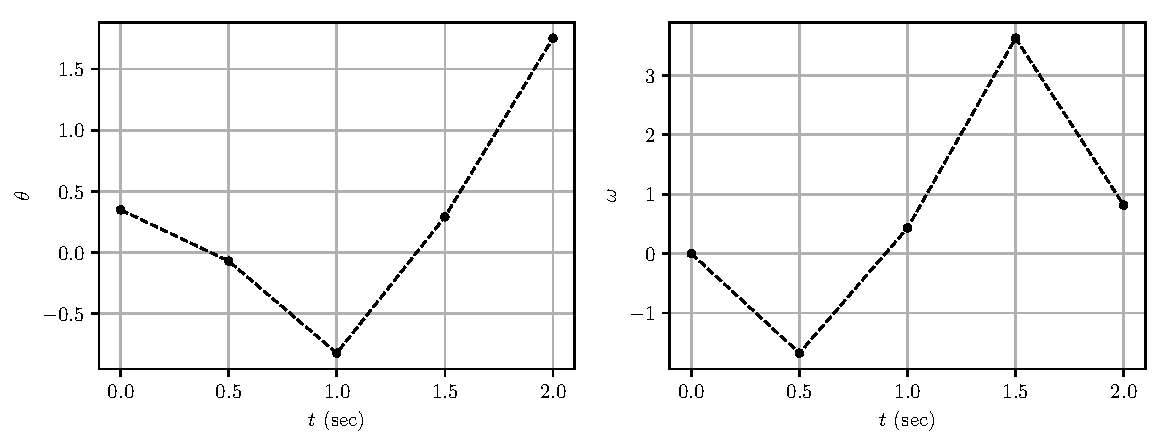
\includegraphics[width=\linewidth]{a}
	\caption{The plotted solution for part a.}
	\label{fig:a}
\end{figure}

\subsection*{Part b: Grid independence with RK-2}

The plot of the relative changes for part b follow in Figure \ref{fig:b}. In this plot, ``all coarse timesteps'' is the maximum relative change over all coarse timesteps for a given variable, and ``$t = 2$ s'' is the relative change in the solution at the final time for a given variable.

\begin{figure}[H]
	\centering
	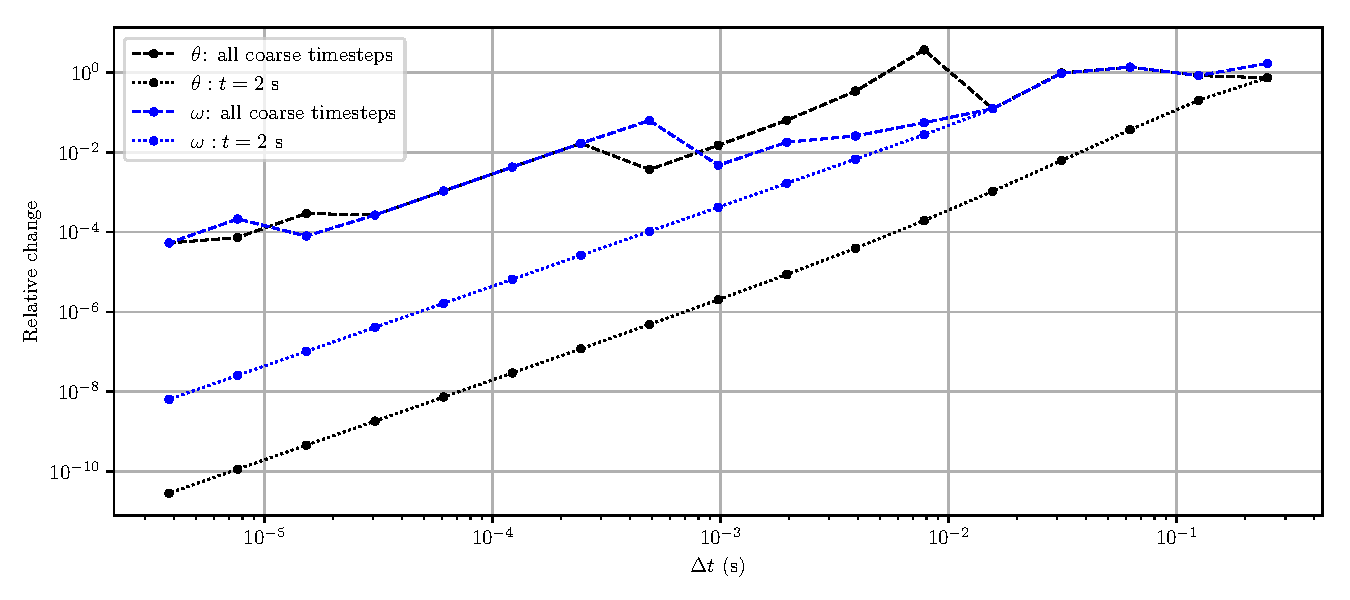
\includegraphics[width=\linewidth]{b}
	\caption{The plotted relative changes used to determine grid independence for part b.}
	\label{fig:b}
\end{figure}

The convergence for a single point in time behaves significantly better than taking the maximum over each solution time. We expect this because the order of accuracy should decrease by one from a point value to a maximum.

\subsection*{Part c: All methods}

The explicit and implicit Euler methods were also utilized at the previously determined grid independent timestep size ($\Delta t = 3.8\times10^{-6}$ s) for part c. The resulting solutions are plotted below in Figure \ref{fig:c}.

\begin{figure}[H]
	\centering
	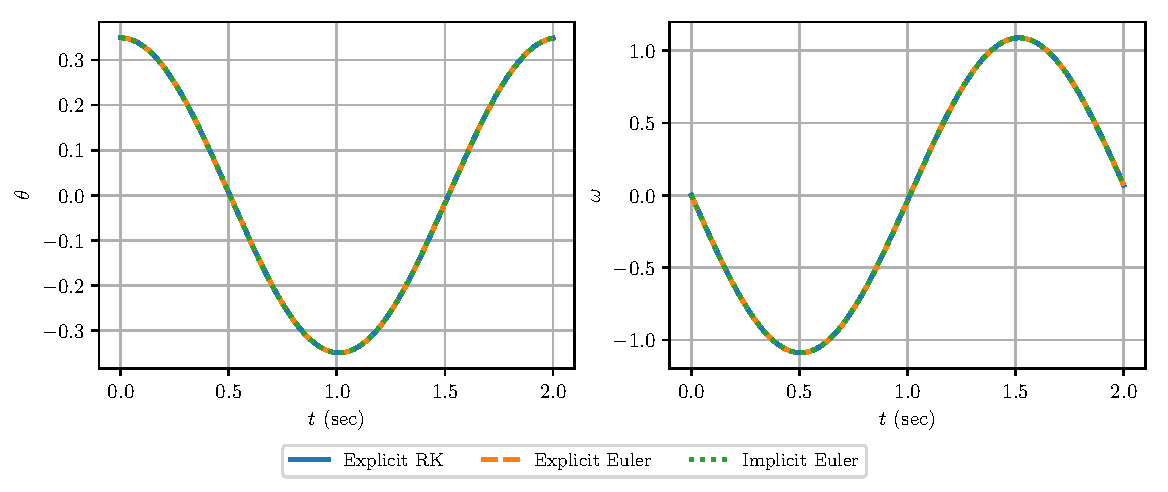
\includegraphics[width=\linewidth]{c}
	\caption{The plotted solutions with $\Delta t = 3.8\times10^{-6}$ s (grid-independent) compared among all methods for part c.}
	\label{fig:c}
\end{figure}

\end{document}
